%!TEX program = xelatex
\documentclass[cn,hazy,blue,10pt,normal]{elegantnote}
\title{The Illustrated Transformer}

\author{作者:Jay Alammar \qquad 原文:\href{https://jalammar.github.io/illustrated-transformer/}{The Illustrated Transformer}}
\institute{}

%\version{2.50}
%\date{\zhdate{2022/12/31}}

\usepackage{array}

\begin{document}
	


\maketitle

\begin{abstract}
	在\href{https://jalammar.github.io/visualizing-neural-machine-translation-mechanics-of-seq2seq-models-with-attention/}{之前的文章}中,我们探讨了深度学习模型中广泛应用的注意力机制。注意力机制是提升神经机器翻译应用性能的关键。本文将聚焦于\textbf{Transformer},这是一个利用注意力机制显著提升模型训练速度的先进模型。在特定任务上,Transformer 甚至超过了谷歌的神经机器翻译模型。但它最大的优势在于适合并行处理。Google Cloud 甚至推荐将 Transformer 作为使用其\href{https://cloud.google.com/tpu/}{Cloud TPU}的参考模型。接下来,我们将深入分析 Transformer 的工作原理。
	
	Transformer 最初在论文\href{https://arxiv.org/abs/1706.03762}{“Attention is All You Need”}中提出,其 TensorFlow 实现可以在 \href{https://github.com/tensorflow/tensor2tensor}{Tensor2Tensor} 包中找到。哈佛大学的 NLP 团队还制作了一个\href{http://nlp.seas.harvard.edu/2018/04/03/attention.html}{配有 PyTorch 实现的论文解读指南}。本文旨在用更浅显的方式逐一介绍这些概念,使非专业人士也能轻松理解。
\end{abstract}

%\centerline{
%  \includegraphics[width=0.2\textwidth]{logo-blue.png}
%}

\section{浅显解读}

首先,我们将这个模型视为一个神秘的黑盒子。在机器翻译应用中,它负责将一种语言的句子转换成另一种语言的翻译。
\begin{figure}[h]
	\centering
	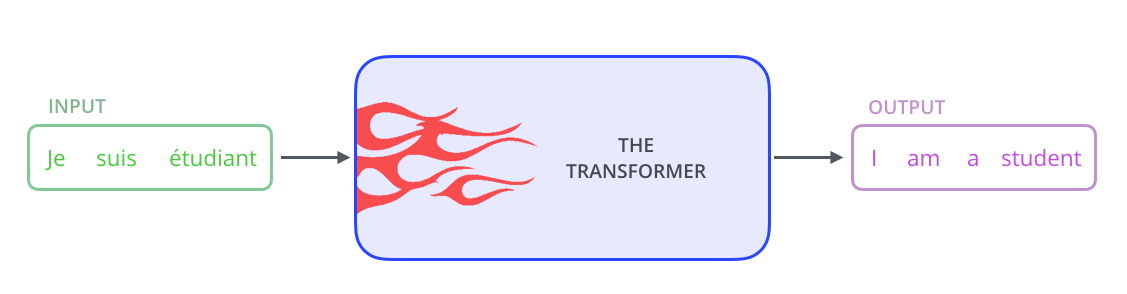
\includegraphics[width=0.75\textwidth]{image/the_transformer_3.png}
\end{figure}

打开这个令人着迷的“擎天柱”盒子,我们发现了编码器(encoder)组件、解码器(decoder)组件,以及它们之间的连接。
\begin{figure}[h]
	\centering
	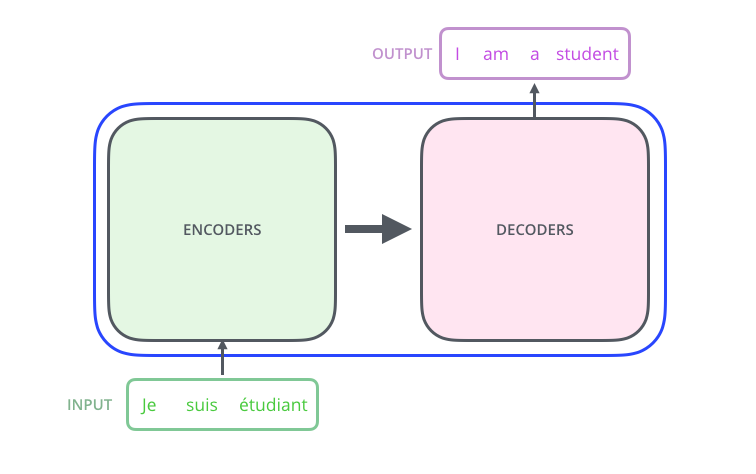
\includegraphics[width=0.5\textwidth]{image/The_transformer_encoders_decoders.png}
\end{figure}

编码器组件由一系列编码器堆叠而成(论文中堆叠了六个,但六并没有什么特别的含义,你可以尝试其他的组合方式)。解码器组件则由同样数量的解码器堆叠而成。
\begin{figure}[!h]
	\centering
	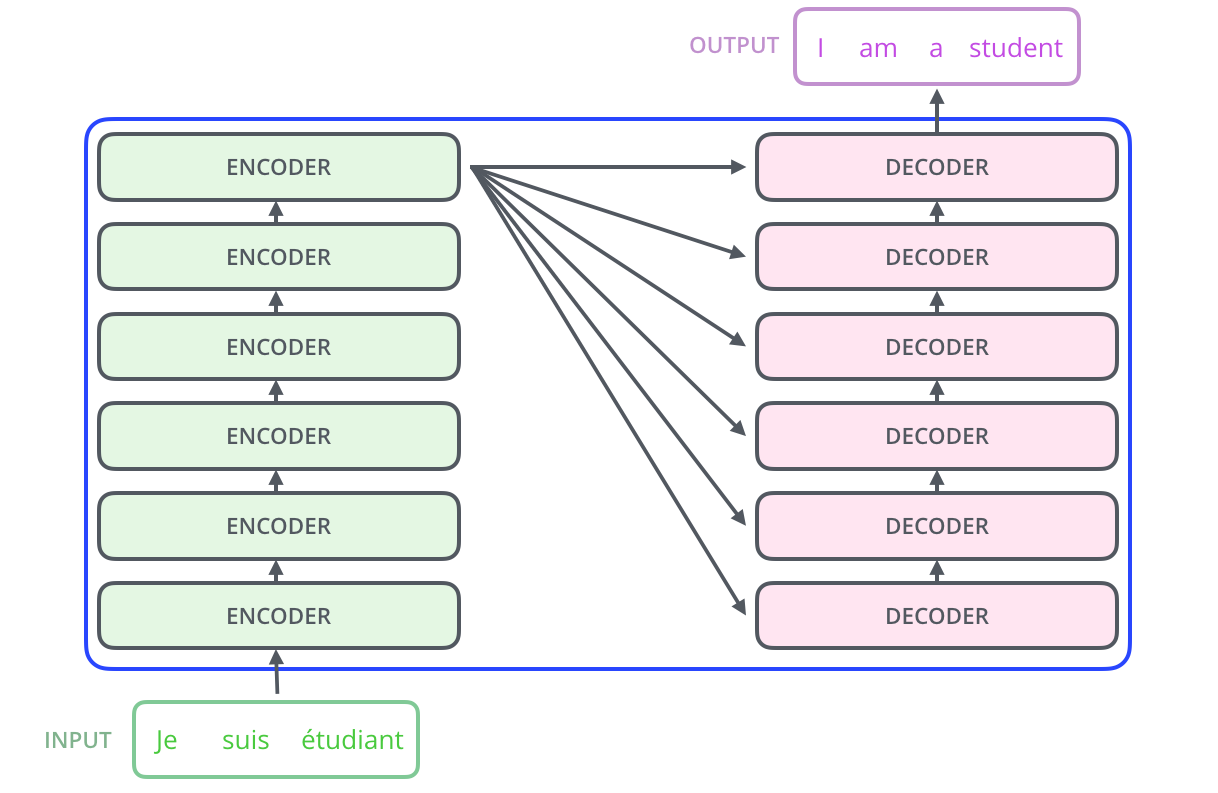
\includegraphics[width=0.5\textwidth]{image/The_transformer_encoder_decoder_stack.png}
\end{figure}

所有的编码器结构相同(但它们并不共享权重)。每个编码器分为两个子层:
\begin{figure}[h]
	\vspace{-10mm}
	\centering
	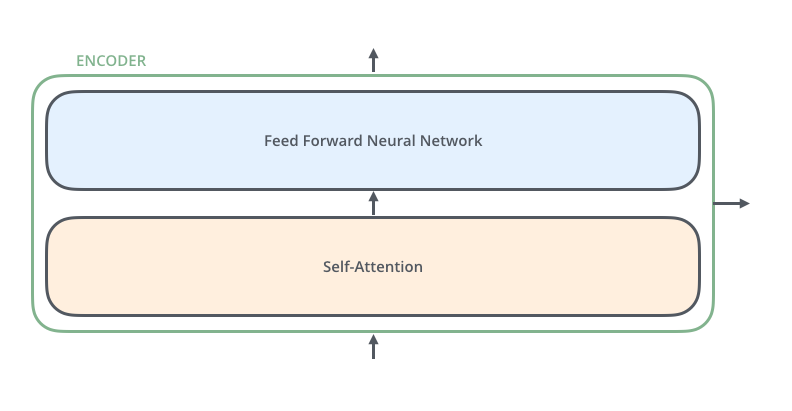
\includegraphics[width=0.5\textwidth]{image/Transformer_encoder.png}
\end{figure}

编码器的输入首先通过一个自注意力(self-attention)层。这个层帮助编码器在对一个特定单词进行编码时,还能注意到输入句子中的其他单词。我们将在后面的文章中深入探讨自注意力层。

自注意力层的输出接着被送入一个前馈神经网络。每个位置都独立应用相同的前馈网络。

解码器包含了这两种层,但在它们之间还有一个额外的注意力层,它帮助解码器关注输入句子中的相关部分,这与序列到序列模型(seq2seq models)中的注意力机制类似。
\begin{figure}[h]
	\centering
	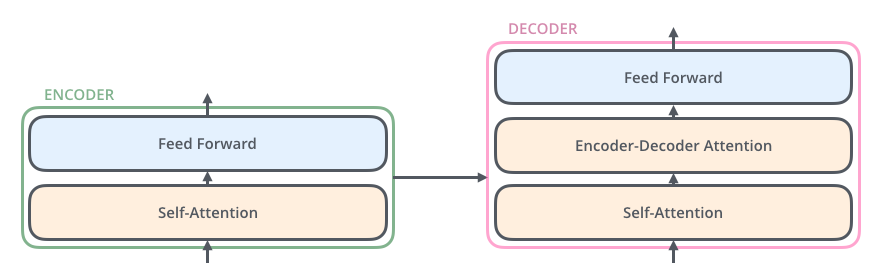
\includegraphics[width=0.5\textwidth]{image/Transformer_decoder.png}
\end{figure}

\section{引入张量到图像中}

现在我们已经了解了模型的主要组成部分,接下来探讨各种向量和张量如何在这些组件之间流动,把经过训练的模型的输入转化为输出。

自然语言处理应用中,我们通常先使用一个\href{https://medium.com/deeper-learning/glossary-of-deep-learning-word-embedding-f90c3cec34ca}{嵌入算法}将每个输入词转化为一个向量。
\begin{figure}[h]
	\centering
	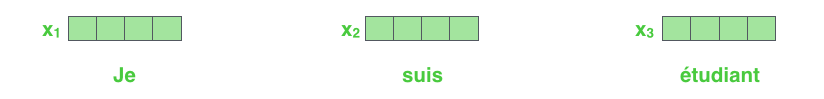
\includegraphics[width=0.75\textwidth]{image/embeddings.png}
	\caption{每个单词被嵌入成一个 512 维的向量,我们用这些简洁的方框来表示这些向量。}
\end{figure}

每个单词被嵌入成一个 512 维的向量,我们用这些简洁的方框来表示这些向量。

嵌入过程仅在最底层的编码器(encoder)中发生。所有编码器共同的特点是它们接收一系列 512 维的向量 - 在底层编码器中,这些向量是词嵌入,而在其他编码器中,则是下方编码器的输出。这个向量列表的长度是一个我们可以设定的超参数,通常是我们训练数据集中最长句子的长度。

在我们的输入序列中嵌入单词后,这些单词会依次通过编码器的两个层级。
\begin{figure}[h]
	\centering
	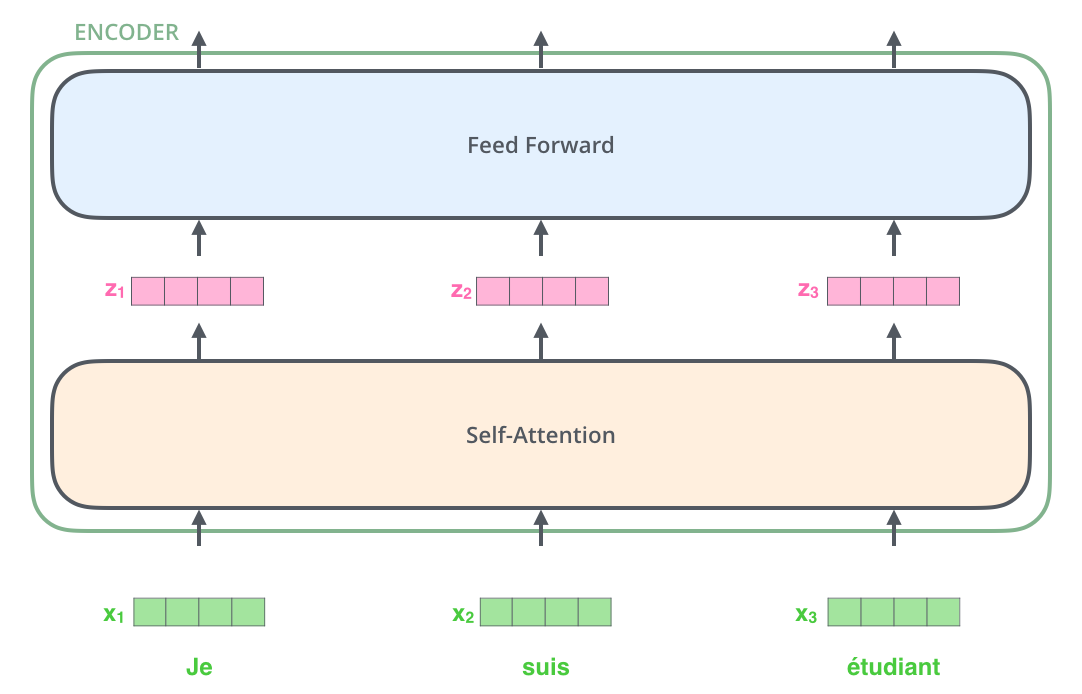
\includegraphics[width=0.5\textwidth]{image/encoder_with_tensors.png}
\end{figure}

这里我们可以看到 Transformer 的一个关键特点,即每个位置上的词都在编码器中沿着自己的路径流动。在自注意力层(self-attention layer)中,这些路径之间存在相互依赖关系。然而,在前馈层(feed-forward layer)中并没有这样的依赖,因此在流经前馈层时,不同的路径可以并行处理。

接下来,我们将使用一个更短的句子作为例子,来观察编码器中每个子层的作用。

\section{现在我们开始编码!}

如我们所述,编码器接收一系列向量作为输入,并对这些向量进行处理。它们首先被传递到一个自注意力层,然后是一个前馈神经网络,最后输出到上方的下一个编码器。

\begin{figure}[htbp]
	\centering
	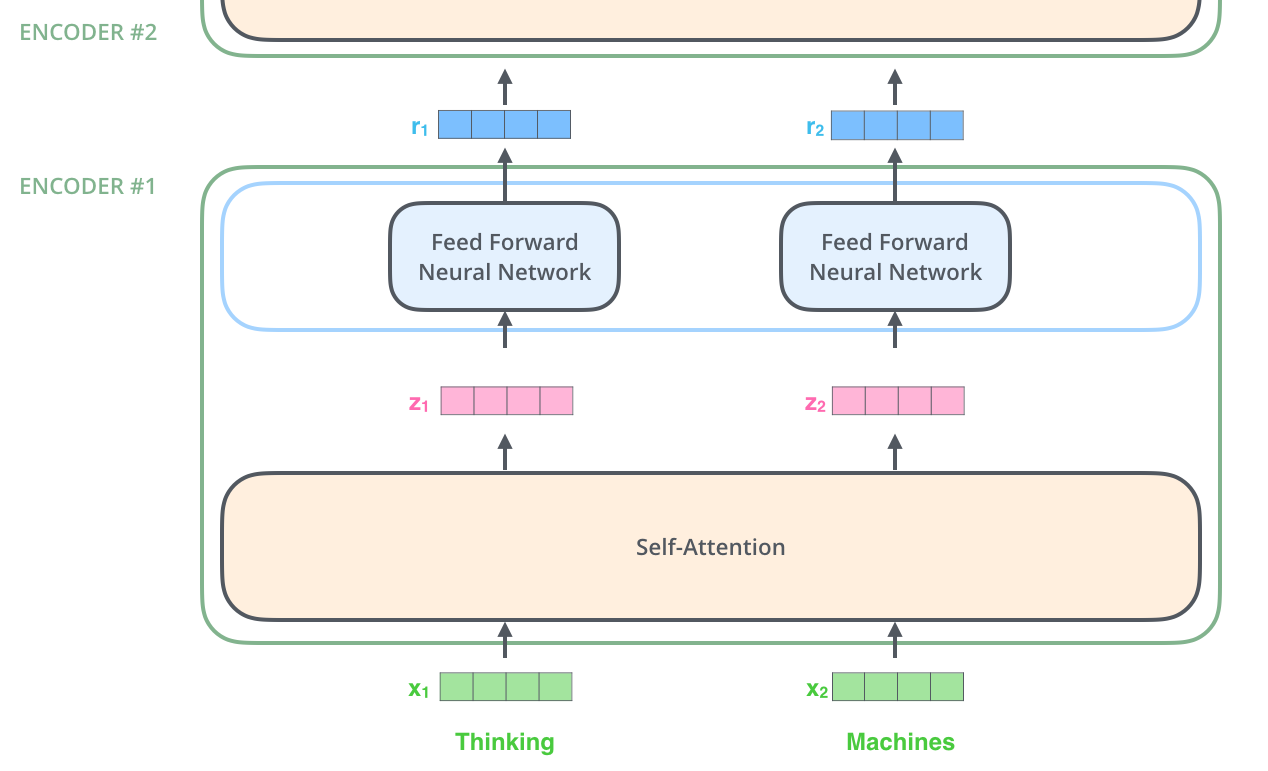
\includegraphics[width=0.5\textwidth]{image/encoder_with_tensors_2.png}
	\caption{每个位置上的词都经历一个自注意力处理过程,随后各自通过同一个前馈神经网络,但每个向量都是独立处理的。
}
\end{figure}

\section{自注意机制 (Self-Attention) 的高层次理解}

提到“自注意机制”这个术语时,不要以为它是一个人人皆知的概念。事实上,我在阅读《Attention is All You Need》这篇论文之前,也是第一次接触到这个概念。我们来浅显地解释一下它的工作原理。

以这样一个待翻译的输入句子为例:
\textbf{The animal didn't cross the street because it was too tired (动物因为太累了,所以它没有穿过街道)}

这句话中的“it”是指什么?是指 street 还是 animal?对人来说这是个简单的问题,但对算法而言就没那么简单了。
在模型处理“it”这个词时,自注意机制使其能将“it”与“animal”联系起来。
当模型逐个处理每个词(输入序列中的每个位置)时,自注意机制使其能够查看输入序列中的其它位置,以寻找有助于更好地理解当前词的线索。

如果你对 RNNs 有所了解,可以将自注意机制想象为类似于 RNN 保持隐藏状态的方式,它将处理过的先前词汇/向量的信息与当前正在处理的词汇结合起来。自注意机制是 Transformer 用于将对其它相关词汇的“理解”融入到当前处理的词汇中的方法。

\begin{figure}[htbp]
	\centering
	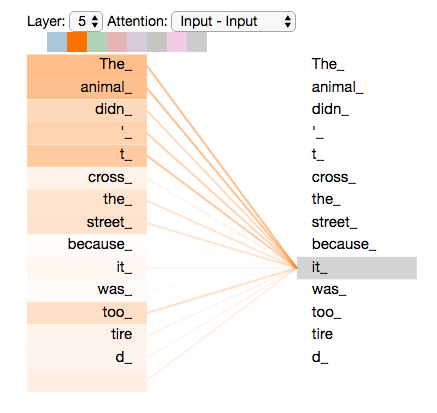
\includegraphics[width=0.4\textwidth]{image/transformer_self-attention_visualization.png}
	\caption{例如,在编码器 \#5(堆栈中的顶层编码器)中处理“it”这个词时,注意力机制的一部分就聚焦在了“animal”上,并将其一部分信息融入到了“it”的编码中。
	}
\end{figure}

你可以访问\href{https://colab.research.google.com/github/tensorflow/tensor2tensor/blob/master/tensor2tensor/notebooks/hello_t2t.ipynb}{Tensor2Tensor 笔记本}来加载一个 Transformer 模型,并通过这个交互式可视化工具来深入了解它。

\section{自注意力详解}

让我们首先了解如何使用向量计算自注意力(Self-Attention),然后探究其如何通过矩阵实际实现。

在计算自注意力的\textbf{第一步},我们需要从编码器的每个输入向量(这里是每个单词的嵌入)生成三个向量:一个查询向量(Query vector)、一个键向量(Key vector)和一个值向量(Value vector)。这些向量是通过将单词嵌入与我们在训练过程中训练出的三个矩阵相乘产生的。

值得注意的是,这些新向量的维度比原始的嵌入向量要小。它们的维度是 64,相比之下,嵌入和编码器的输入/输出向量的维度为 512。选择更小的维度是一种架构上的决定,目的是为了让多头注意力(Multiheaded Attention)的计算在大多数情况下保持相对固定。

\begin{figure}[htbp]
	\centering
	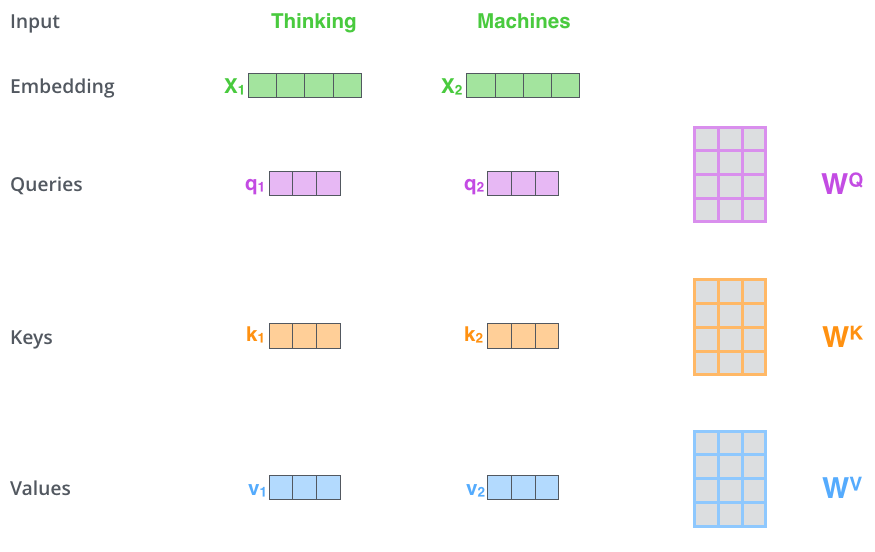
\includegraphics[width=0.5\textwidth]{image/transformer_self_attention_vectors.png}
	\caption{例如,通过 $W^Q$ 权重矩阵乘以 $x_1$ 可以得到 $q_1$,即与该单词相关联的“查询”向量。这样,我们就为输入句子中的每个单词创建了一个“查询”、“键”和“值”的投影。
	}
\end{figure}

那么,这些“查询”、“键”和“值”向量究竟是什么呢?

它们是帮助我们计算和理解注意力机制的抽象概念。当你阅读下面关于注意力如何计算的部分时,你将更深入地理解这些向量各自的角色。

在自注意力的计算中的\textbf{第二步},我们需要计算一个得分。以这个例子中的第一个单词“Thinking”为例,我们要为这个单词与输入句子中的每个单词进行得分。这个得分决定了在编码某个位置的单词时,我们应该把多少注意力放在输入句子的其他部分。

这个得分是通过计算查询向量与相应单词的键向量的点积来得出的。因此,如果我们正在处理位置\#1 的单词“Thinking”的自注意力,第一个得分将是 $q_1$ 和 $k_1$ 的点积,第二个得分则是 $q_1$ 和 $k_2$ 的点积。

\begin{figure}[htbp]
	\centering
	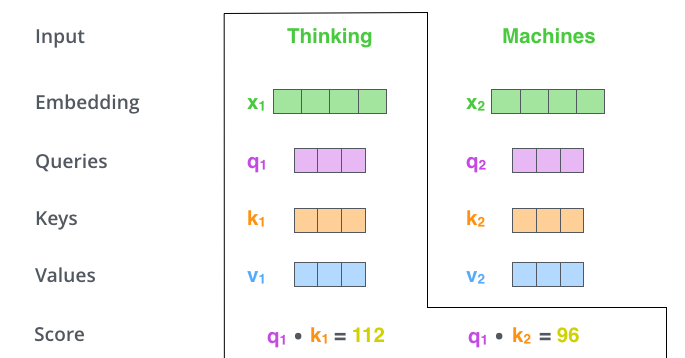
\includegraphics[width=0.5\textwidth]{image/transformer_self_attention_score.png}
\end{figure}

\textbf{第三步和第四步} 是将得分除以 8,这是因为在论文中键向量的维度是 64,8 是其平方根。这样处理可以使得梯度更加稳定。虽然还有其他可能的数值,但 8 通常是默认选择。接着,结果会经过一个 softmax 函数处理。softmax 函数的作用是将得分转换为正数,并且它们的总和为 1。

\begin{figure}[htbp]
	\centering
	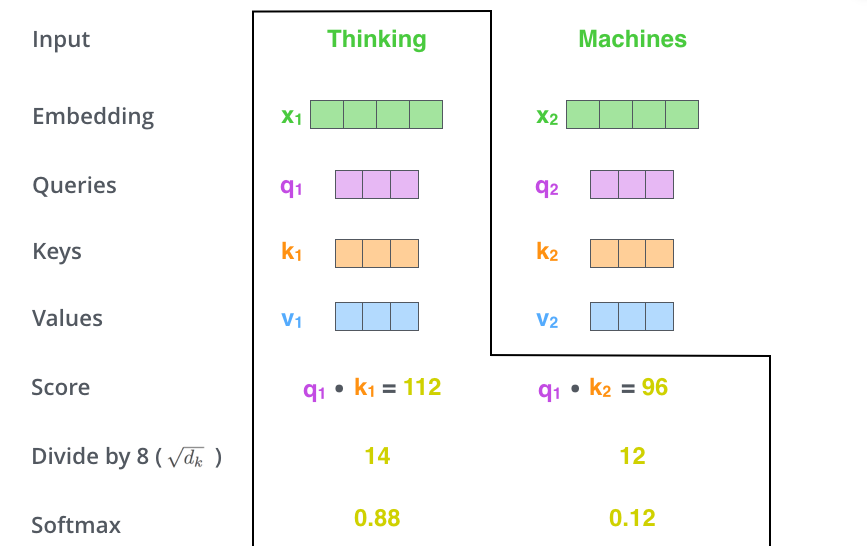
\includegraphics[width=0.5\textwidth]{image/self-attention_softmax.png}
\end{figure}

这个经过 softmax 函数处理的分数决定了在这个位置每个词的表达程度。一般来说,该位置的词会获得最高的 softmax 分数,但有时关注与当前词相关的其他词也是重要的。

\textbf{第五步} 是将每个值向量与其对应的 softmax 分数相乘,为接下来的累加做准备。这一步的关键思想是通过权重来强调我们关注的词汇,同时减弱与之无关的词汇(比如,将其与很小的数字如 0.001 相乘)。

\textbf{第六步} 是将这些加权后的值向量求和。这样就得到了在这个位置(对于第一个词而言)的自我注意力层的输出结果。

\begin{figure}[ht]
	\centering
	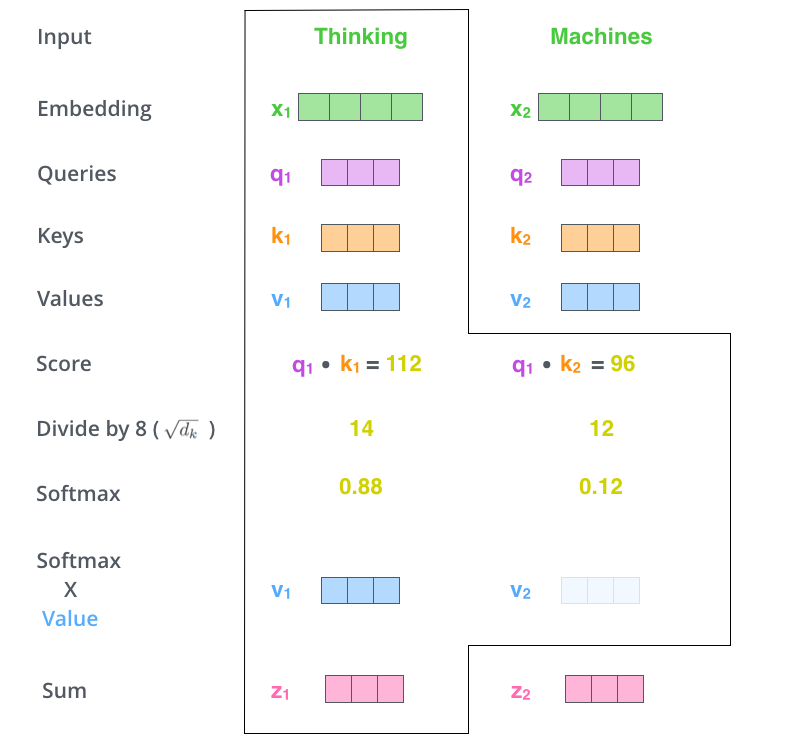
\includegraphics[width=0.5\textwidth]{image/self-attention-output.png}
\end{figure}

至此,自我注意力的计算过程就完成了。得到的向量接下来将被送入前馈神经网络。不过,在实际的实现中,为了提高处理速度,这一计算过程是以矩阵的形式进行的。现在我们已经理解了在单词层面上的计算直觉,下面就来看看矩阵形式的计算。

\section{自注意力的矩阵计算}

\textbf{第一步},我们需要计算查询 (Query), 键 (Key) 和 值 (Value) 矩阵。这个过程包括将我们的嵌入数据整合到一个名为 $X$ 的矩阵中,然后用我们训练出的权重矩阵($W^Q$、$W^K$、$W^V$)来乘以它。

\begin{figure}[ht]
	\centering
	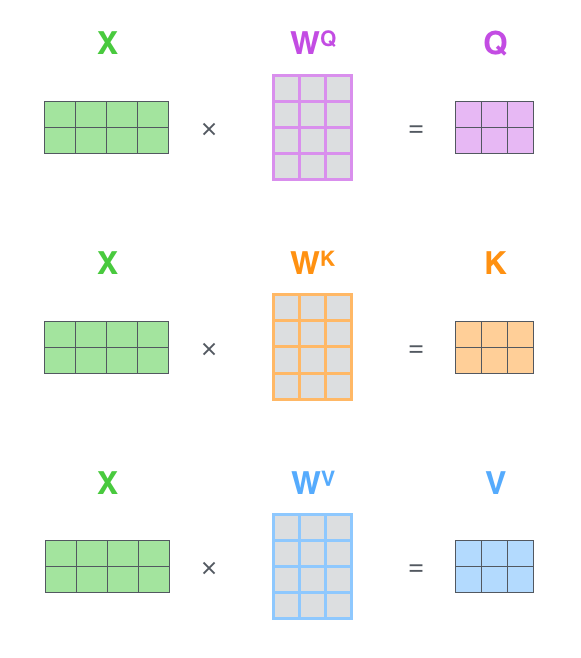
\includegraphics[width=0.45\textwidth]{image/self-attention-matrix-calculation.png}
	\caption{在 X 矩阵中,每一行代表输入句子中的一个词。我们可以看到嵌入向量(512,即图中的 4 个方块)和查询/键/值向量(64,即图中的 3 个方块)之间的尺寸差异。}
\end{figure}

\textbf{最后一步},在处理矩阵时,我们可以用一个公式来简化自注意力层输出计算的第二步到第六步的过程。

\begin{figure}[ht]
	\vspace{-10mm}
	\centering
	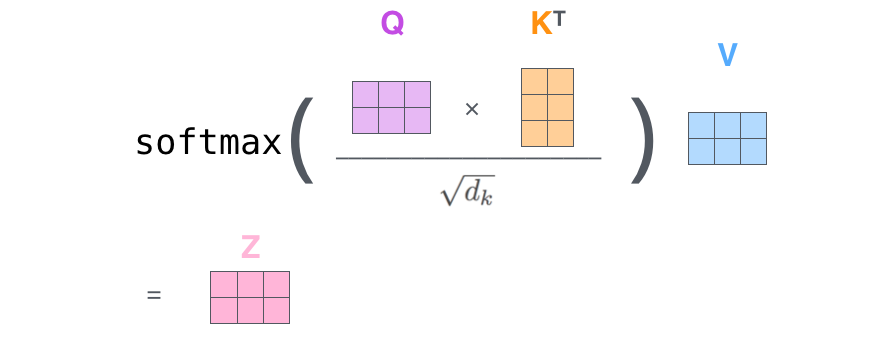
\includegraphics[width=0.5\textwidth]{image/self-attention-matrix-calculation-2.png}
	\caption{自注意力计算的矩阵表示形式}
\end{figure}

\section{多头注意力机制}

该论文进一步优化了自注意力层,引入了一种名为“多头”注意力的机制。这种机制通过两种方式增强了注意力层的性能:
\begin{itemize}
	\item 它增强了模型对不同位置的关注能力。例如,在前述例子中,尽管 z1 包含了一些其他编码的信息,但可能主要受到所对应单词的影响。在翻译如“The animal didn't cross the street because it was too tired”这样的句子时,明确“it”指代的是哪个词非常关键。
	\item 它为注意力层创造了多个“表示子空间”。在多头注意力的帮助下,我们不仅拥有一组,而是多组查询(Query)/键(Key)/值(Value)权重矩阵。例如,Transformer 使用了八个注意力头,因此对于每个编码器/解码器,我们会有八组这样的矩阵。这些矩阵最初是随机初始化的,经过训练后,每组矩阵会将输入的嵌入(或来自下层编码器/解码器的向量)映射到一个不同的表示子空间。
\end{itemize}

\begin{figure}[ht]
	\centering
	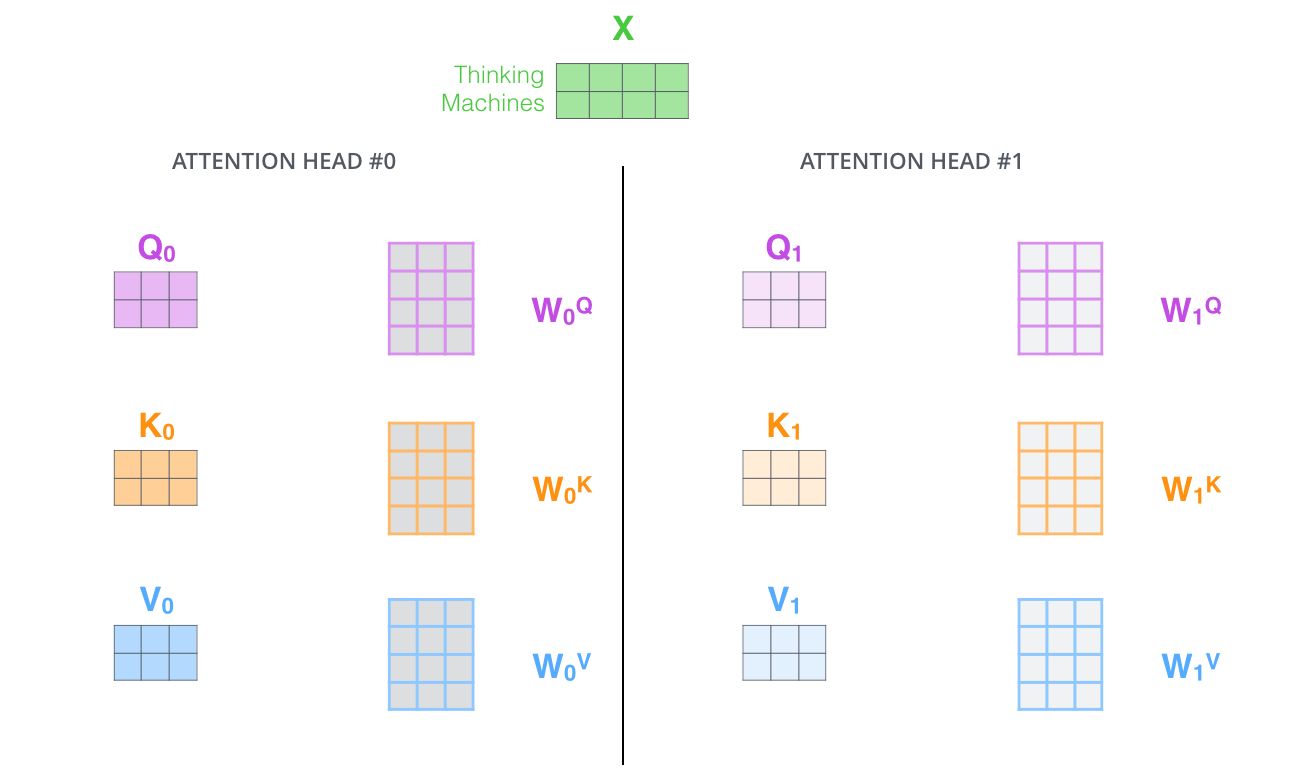
\includegraphics[width=0.5\textwidth]{image/transformer_attention_heads_qkv.png}
	\caption{在多头注意力机制中,我们为每个头维护独立的查询(Q)/键(K)/值(V)权重矩阵,从而得到不同的 Q/K/V 矩阵。我们像之前那样,将输入 X 与 $W^Q/W^K/W^V$ 矩阵相乘,以产生 Q/K/V 矩阵。}
\end{figure}

如果我们按照上述方法进行相同的自注意力计算,但使用不同的权重矩阵重复八次,我们最终会得到八个不同的 Z 矩阵。

\begin{figure}[ht]
	\centering
	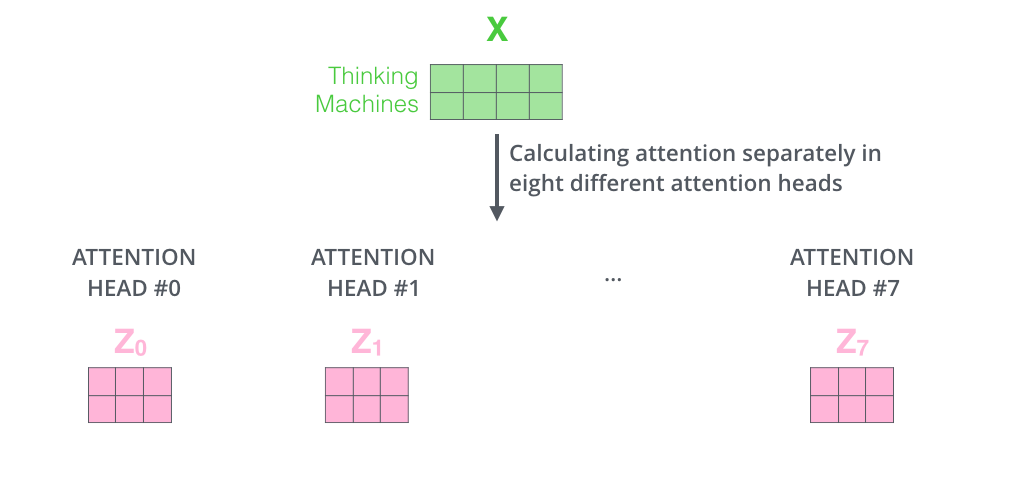
\includegraphics[width=0.5\textwidth]{image/transformer_attention_heads_z.png}
\end{figure}

这就带来了一个挑战:前馈层原本期望得到的是一个单一矩阵(即每个词对应一个向量),而非八个矩阵。因此,我们需要一种方法将这八个矩阵合并为一个。

我们如何实现这一点呢?我们将这些矩阵连结起来,然后用一个额外的权重矩阵 WO 进行乘法运算。

\begin{figure}[ht]
	\centering
	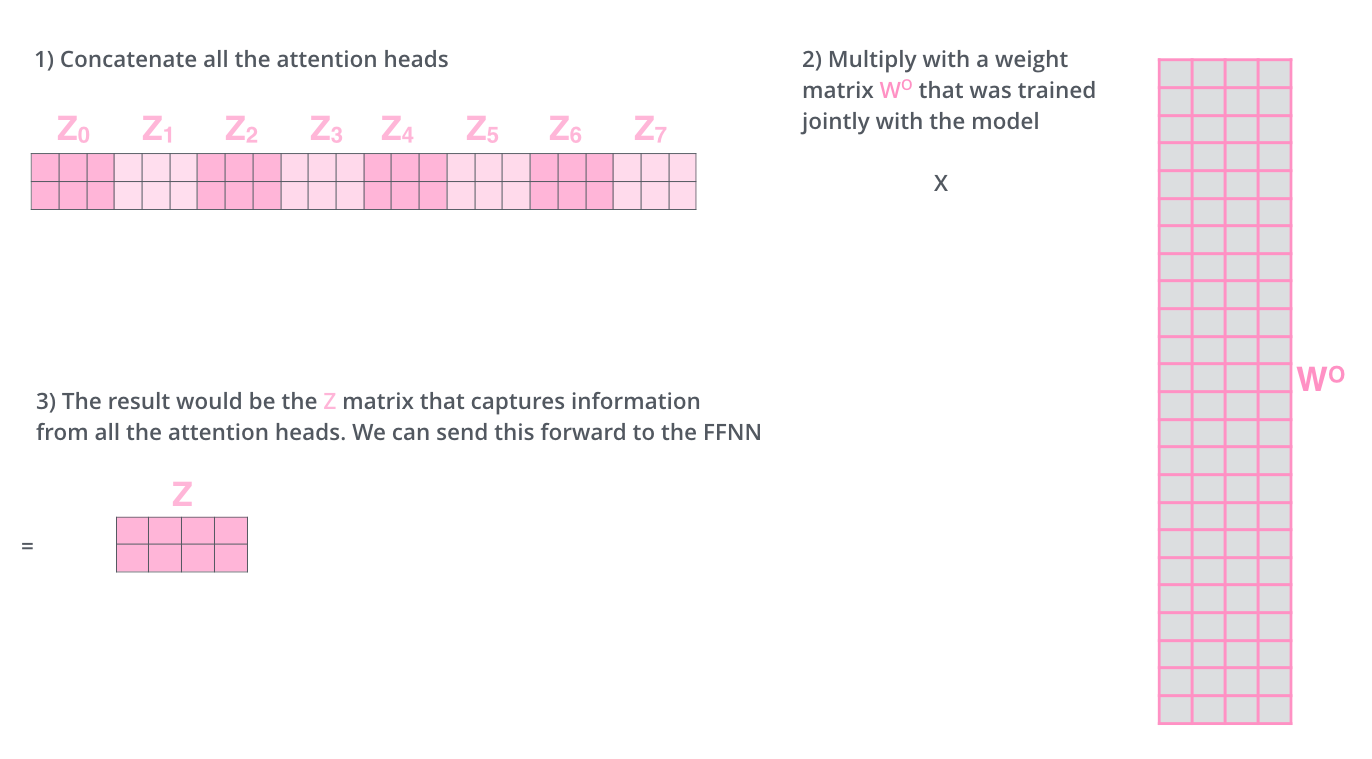
\includegraphics[width=0.5\textwidth]{image/transformer_attention_heads_weight_matrix_o.png}
\end{figure}

这基本上就是多头自注意力的全部内容。尽管涉及许多矩阵,但它们构成了一个完整的视觉表现,让我们能够在一个地方一览无余。

\begin{figure}[ht]
	\centering
	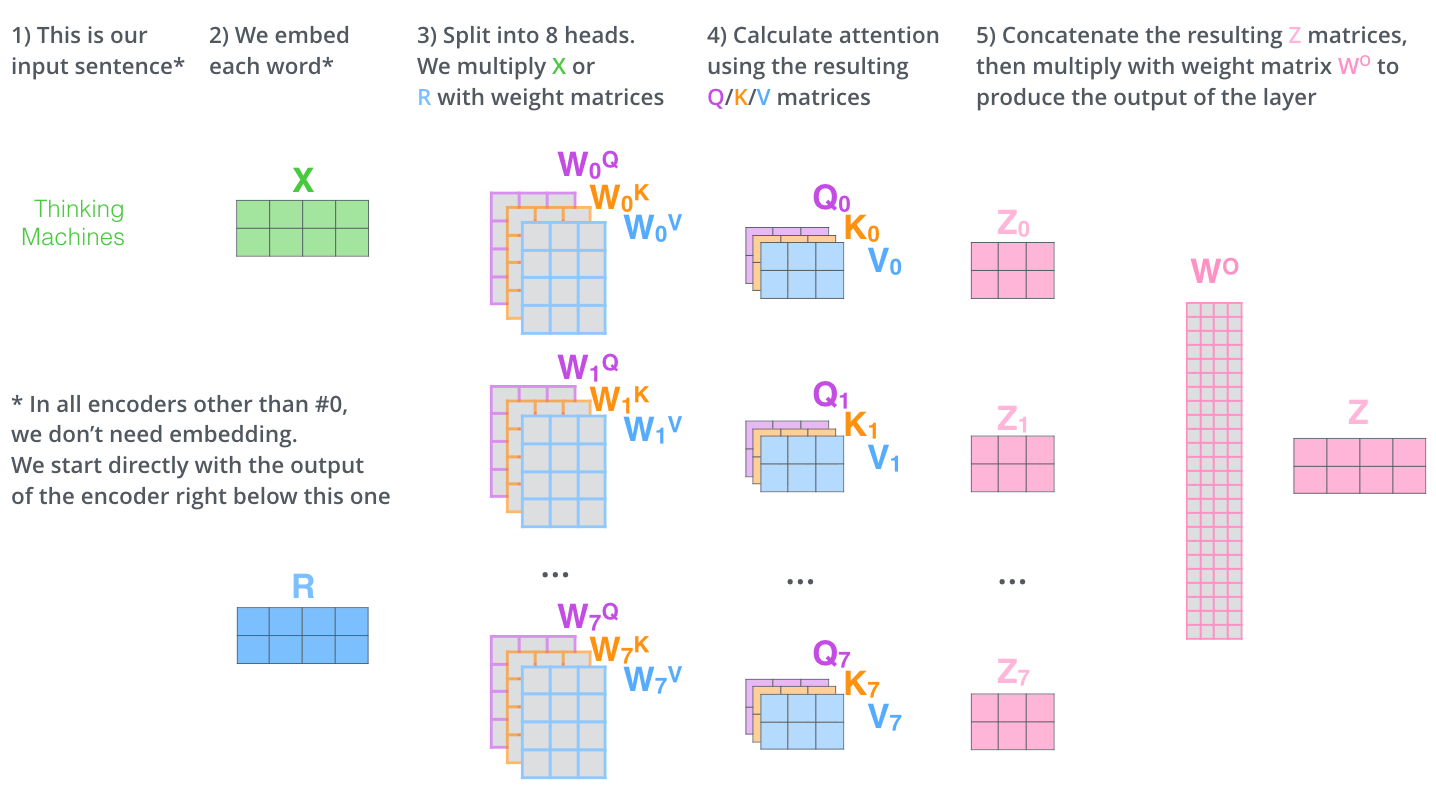
\includegraphics[width=0.5\textwidth]{image/transformer_multi-headed_self-attention-recap.png}
\end{figure}

现在我们已经介绍了注意力机制中的头部构成,让我们重新审视之前的例子,观察在我们的例句中对“it”这个词进行编码时,不同的注意力部分分别聚焦在何处:
\begin{figure}[ht]
	\centering
	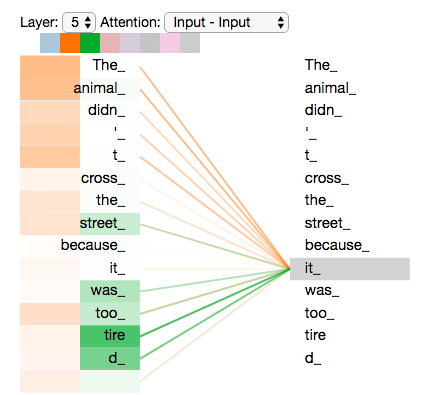
\includegraphics[width=0.5\textwidth]{image/transformer_self-attention_visualization_2.png}
	\caption{在对“it”进行编码时,其中一个注意力部分主要关注于“the animal”,而另一个则聚焦于“tired” —— 这就意味着,模型中“it”这个词的理解融合了对“animal”和“tired”这两个词的理解。}
\end{figure}

然而,当我们把所有注意力部分都考虑进来时,整个情景就变得不那么容易解读了:
\begin{figure}[ht]
	\centering
	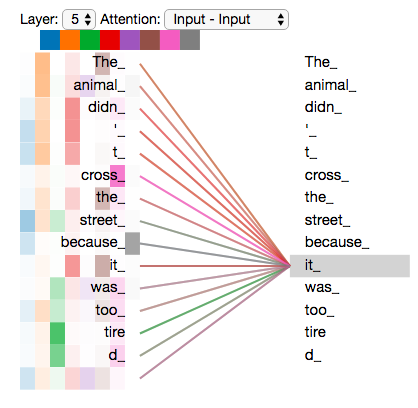
\includegraphics[width=0.5\textwidth]{image/transformer_self-attention_visualization_3.png}
\end{figure}

\newpage

\section{利用位置编码来表达序列中单词的顺序}

到目前为止,我们对模型的描述中缺少的一个方面是如何考虑输入序列中单词的顺序。

为了解决这个问题,Transformer 为每个输入嵌入加入了一个特定的向量。这些向量遵循模型学习到的一个特殊模式,这有助于模型确定每个单词的位置,或序列中不同单词间的距离。这样做的想法是,通过将这些值添加到嵌入中,一旦它们被映射到 Q/K/V 向量并在点积注意力机制中使用,便能够在嵌入向量之间提供有意义的距离。

\begin{figure}[ht]
	\centering
	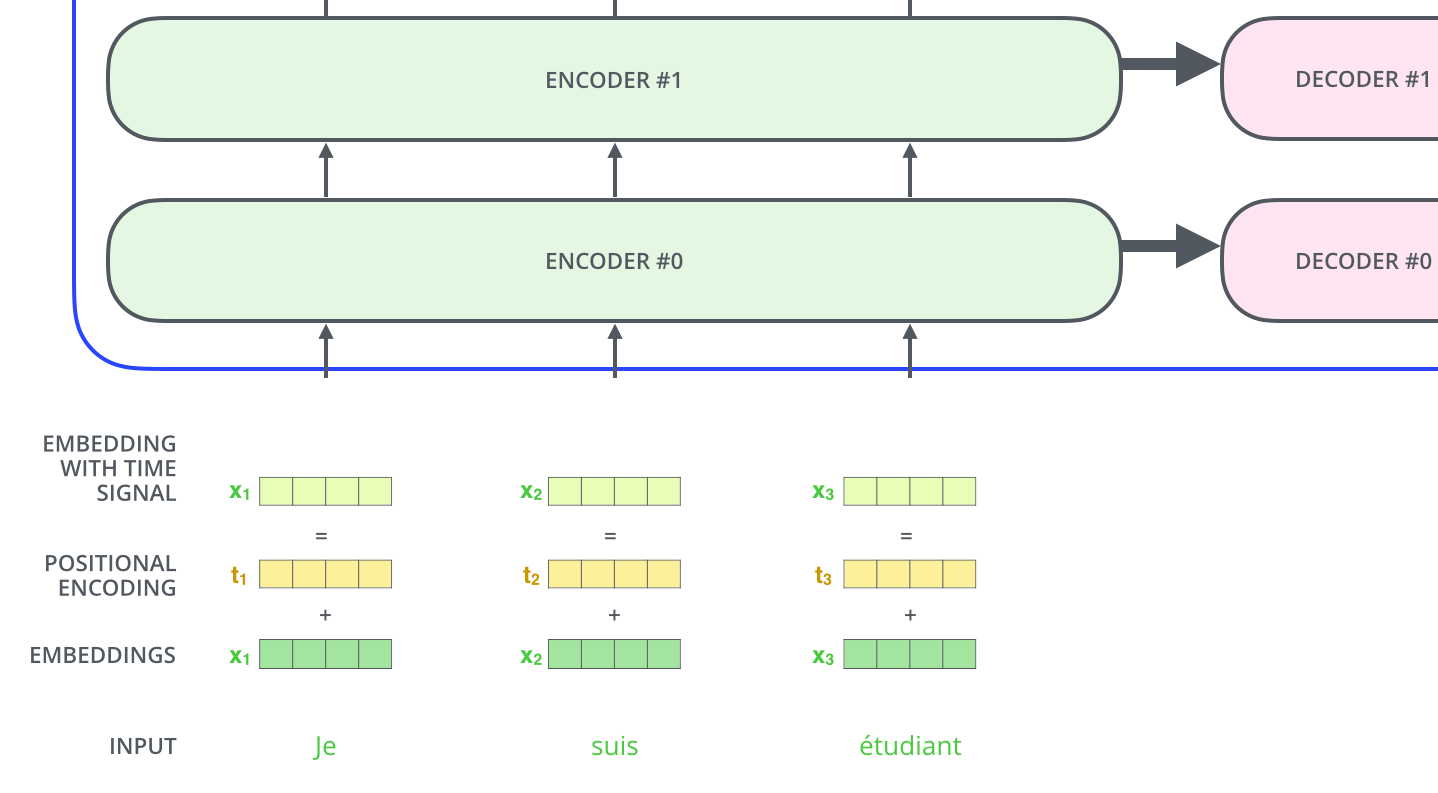
\includegraphics[width=0.5\textwidth]{image/transformer_positional_encoding_vectors.png}
	\caption{为了让模型理解单词的顺序,我们添加了位置编码向量,这些向量的值遵循一个特定的模式。}
\end{figure}

假设嵌入的维度为 4,实际的位置编码可能如下所示:

\begin{figure}[ht]
	\centering
	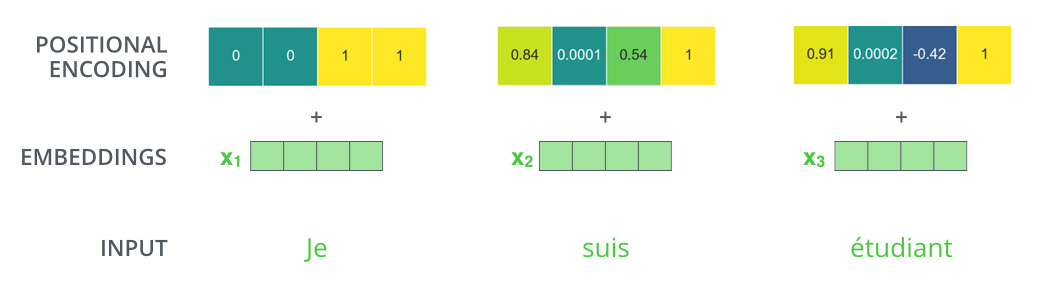
\includegraphics[width=0.5\textwidth]{image/transformer_positional_encoding_example.png}
	\caption{一个维度为 4 的位置编码的实际示例}
\end{figure}

这种模式看起来可能是什么样的?

在下图中,每一行都代表一个向量的位置编码。因此,第一行是我们会添加到输入序列中第一个单词嵌入的向量。每行包含 512 个值,这些值都介于 1 和 -1 之间。我们使用颜色编码使模式更为明显。

\begin{figure}[ht]
	\centering
	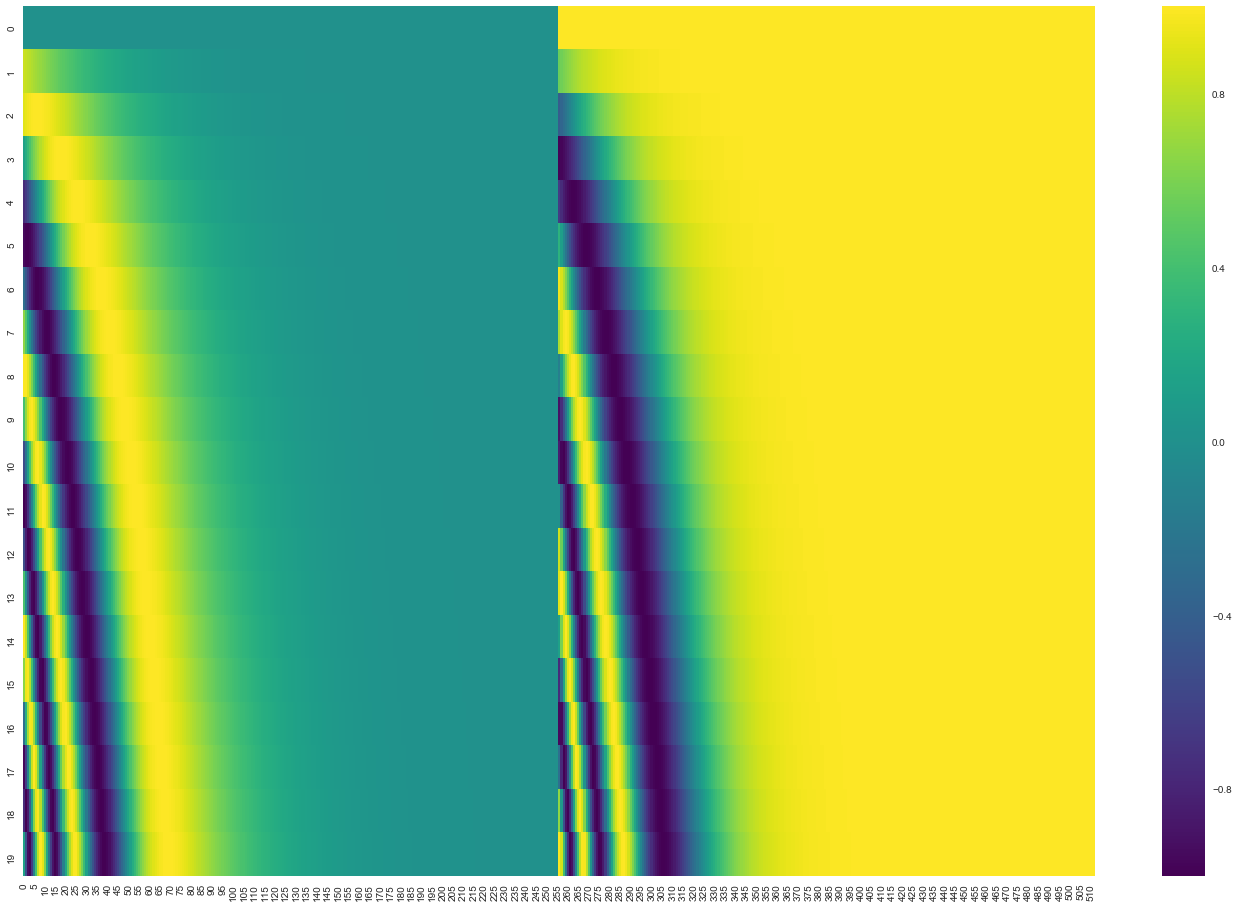
\includegraphics[width=0.65\textwidth]{transformer_positional_encoding_large_example.png}
	\caption{20 个单词(行)和 512 维嵌入大小(列)的位置编码的真实示例。你可以看到图中央分成两半,这是因为左半部的值由一个函数生成(该函数使用正弦波),而右半部则由另一个函数生成(使用余弦波)。然后这些值被合并,形成每个位置编码向量。}
\end{figure}

论文中(第 3.5 节)描述了位置编码的公式。你可以在 \href{https://github.com/tensorflow/tensor2tensor/blob/23bd23b9830059fbc349381b70d9429b5c40a139/tensor2tensor/layers/common_attention.py}{`get\_timing\_signal\_1d()'}中找到生成位置编码的代码。这种方法并非位置编码的唯一方式,但其优势在于能够处理超出训练集中任何句子长度的新序列(比如,训练模型需要翻译一个比训练集中任何句子都长的句子时)。

**2020 年 7 月更新:** 上述的位置编码是基于 Transformer 的 Tensor2Tensor 实现。论文中展示的方法略有差异,它不是直接连接,而是将两种信号交织在一起。下图展示了这种编码的样子。\href{https://github.com/jalammar/jalammar.github.io/blob/master/notebookes/transformer/transformer_positional_encoding_graph.ipynb}{点击此处获取生成该编码的代码}:

\begin{figure}[ht]
	\vspace{-10mm}
	\centering
	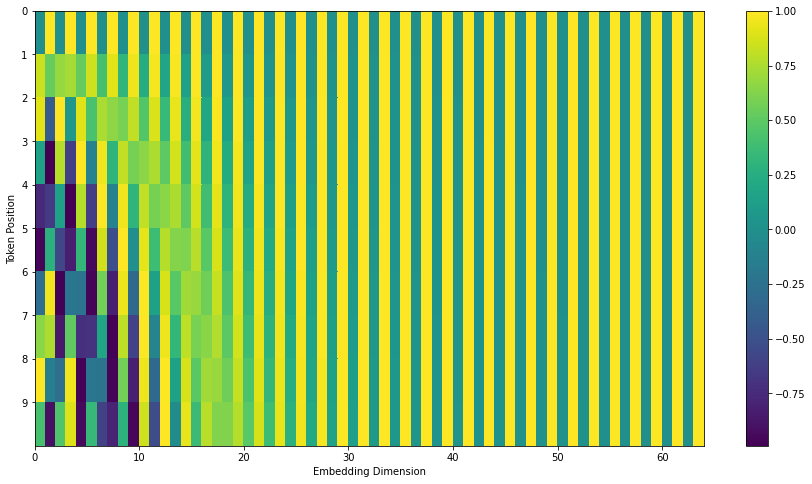
\includegraphics[width=0.65\textwidth]{image/attention-is-all-you-need-positional-encoding.png}
\end{figure}

\section{残差}

在编码器的架构中,有一个重要细节需要说明:编码器的每个子层(比如自注意力 (self-attention)、前馈神经网络 (ffnn))都有一个残差连接,随后还有一个层正规化 (layer-normalization) 步骤。

\begin{figure}[ht]
	\centering
	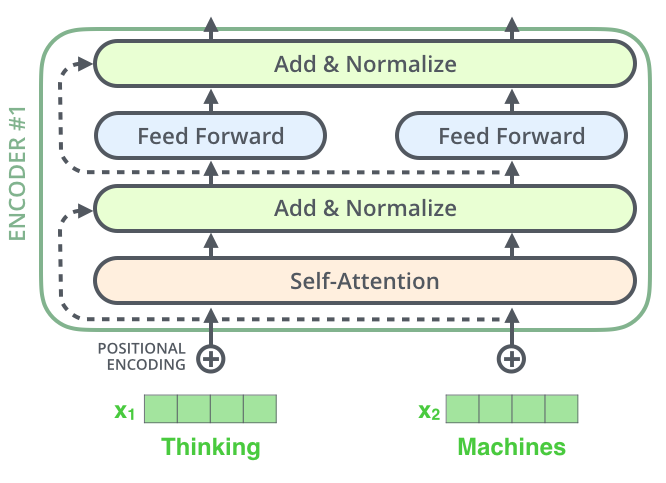
\includegraphics[width=0.5\textwidth]{image/transformer_resideual_layer_norm.png}
\end{figure}

如果我们将自注意力相关的向量和层正规化操作可视化,效果如下图所示:

\begin{figure}[ht]
	\centering
	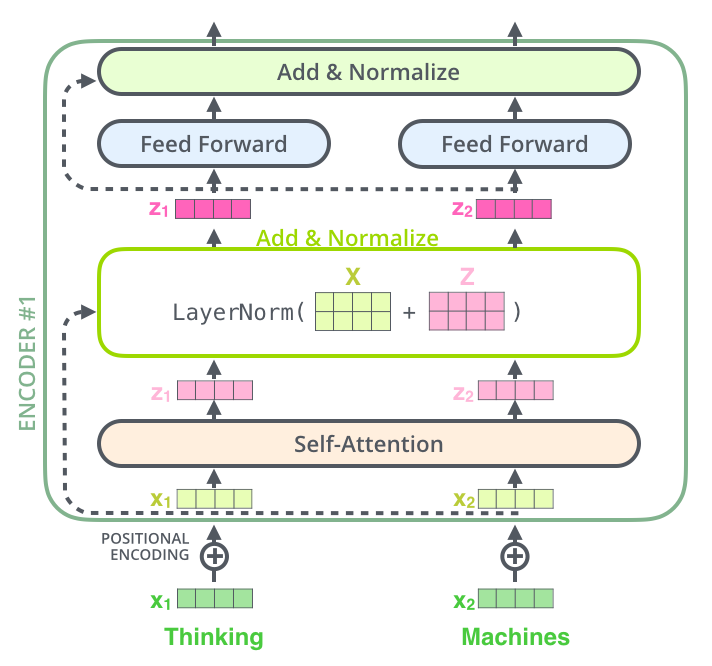
\includegraphics[width=0.5\textwidth]{image/transformer_resideual_layer_norm_2.png}
\end{figure}

解码器的子层同样遵循这一原则。如果我们设想一个由两个堆叠的编码器和解码器组成的 Transformer,其结构大致如下所示:

\begin{figure}[ht]
	\centering
	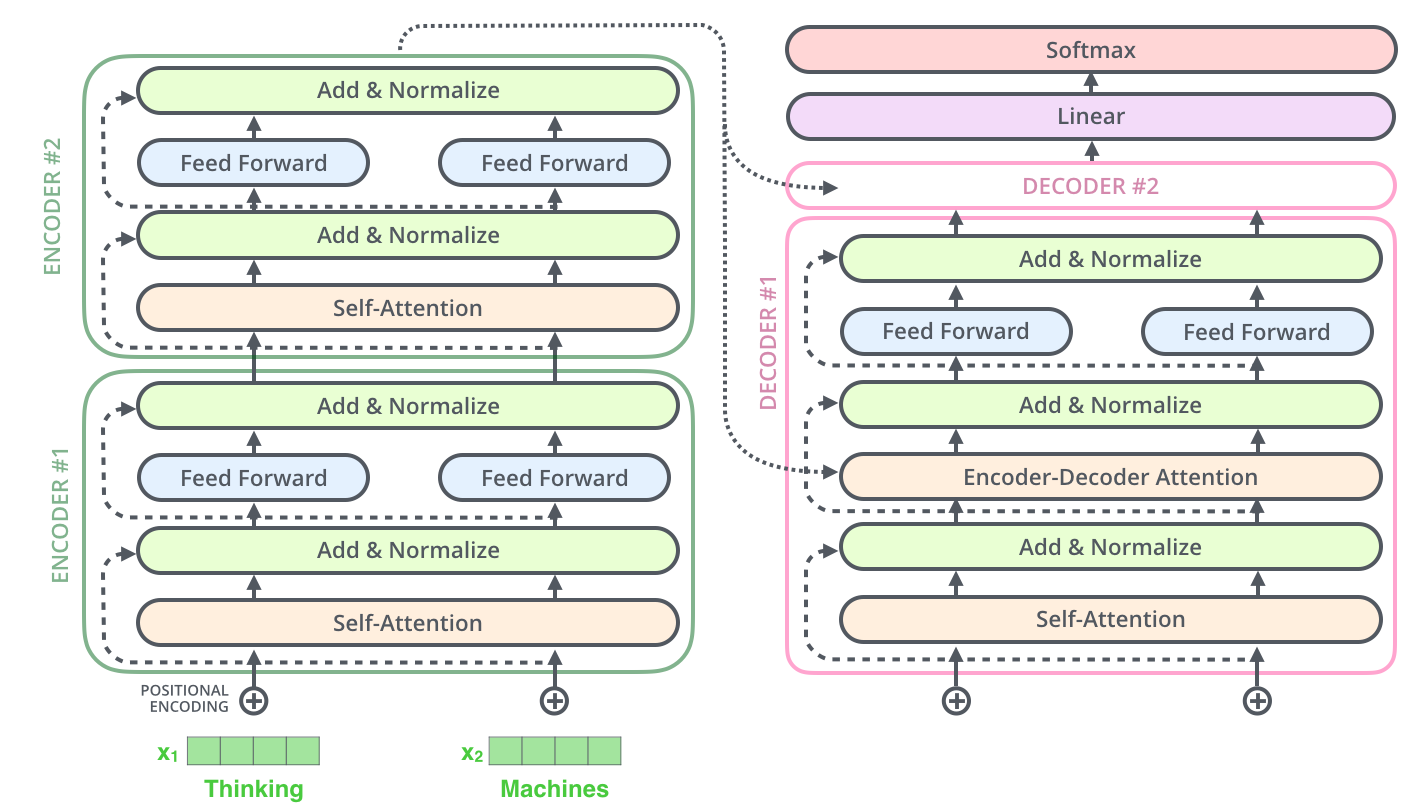
\includegraphics[width=0.65\textwidth]{image/transformer_resideual_layer_norm_3.png}
\end{figure}

\newpage

\section{解码器侧}

在介绍了编码器侧的大部分概念后,我们同样对解码器的组件如何工作有了基本了解。但让我们来看看它们是如何协同工作的。

首先,编码器处理输入序列。然后,顶层编码器的输出被转换成一组注意力向量 K 和 V,用于解码器的““编码器 - 解码器注意力“层,帮助解码器聚焦于输入序列中的关键部分:

\begin{figure}[ht]
	\centering
	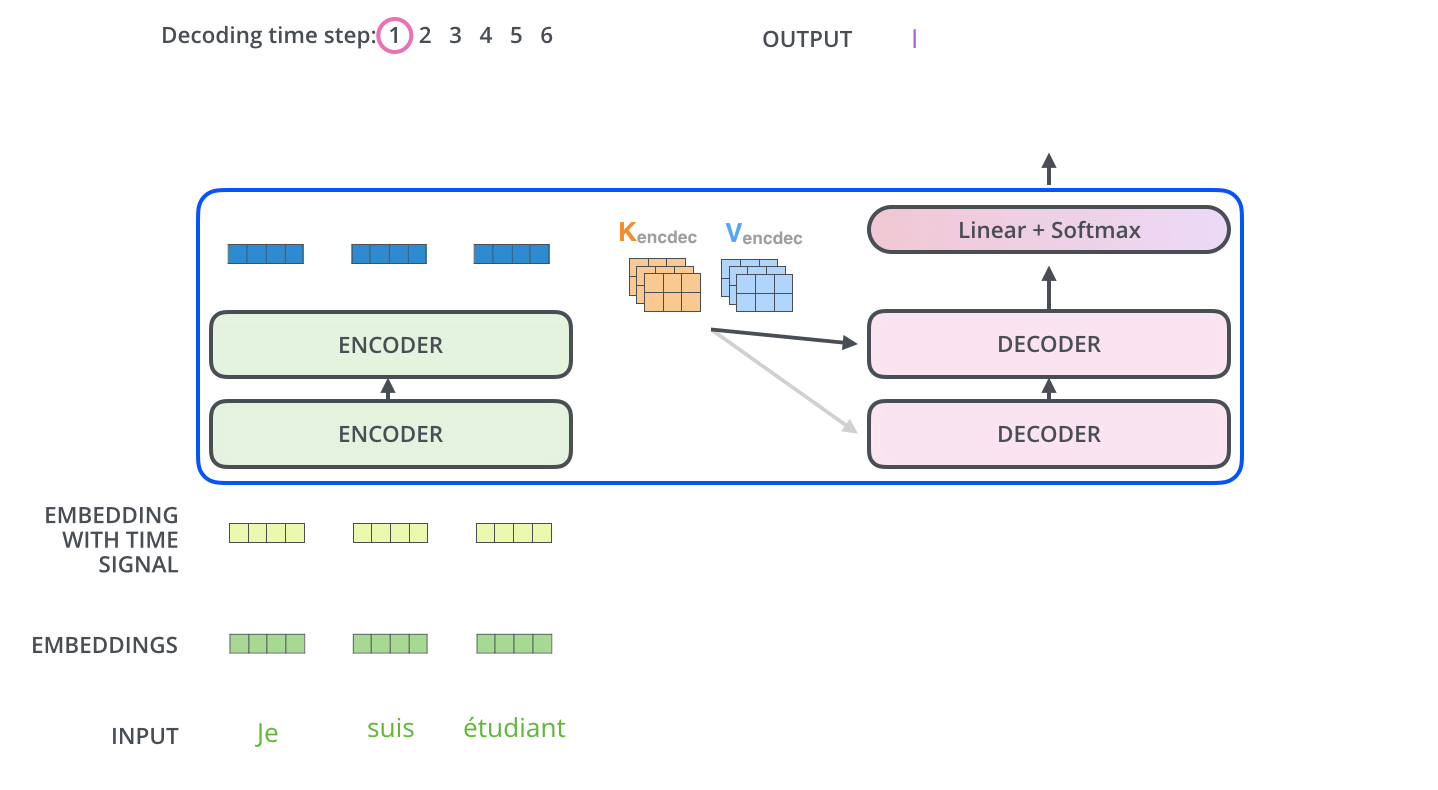
\includegraphics[width=0.5\textwidth]{image/transformer_decoding_1.png}
	\caption{在完成编码阶段之后,我们进入解码阶段。解码阶段的每一步都会产生输出序列(本例中为英语翻译句子)中的一个元素。
	}
\end{figure}

此过程重复进行,直至遇到一个特殊的结束符号,标志着 Transformer 解码器完成了它的输出。每个步骤的输出都会作为下一个时间步骤的底部解码器的输入,并且解码器会像编码器那样逐层传递解码结果。我们还会像处理编码器输入那样,对这些解码器输入进行嵌入并加入位置编码,以标明每个单词的位置。

\begin{figure}[ht]
	\centering
	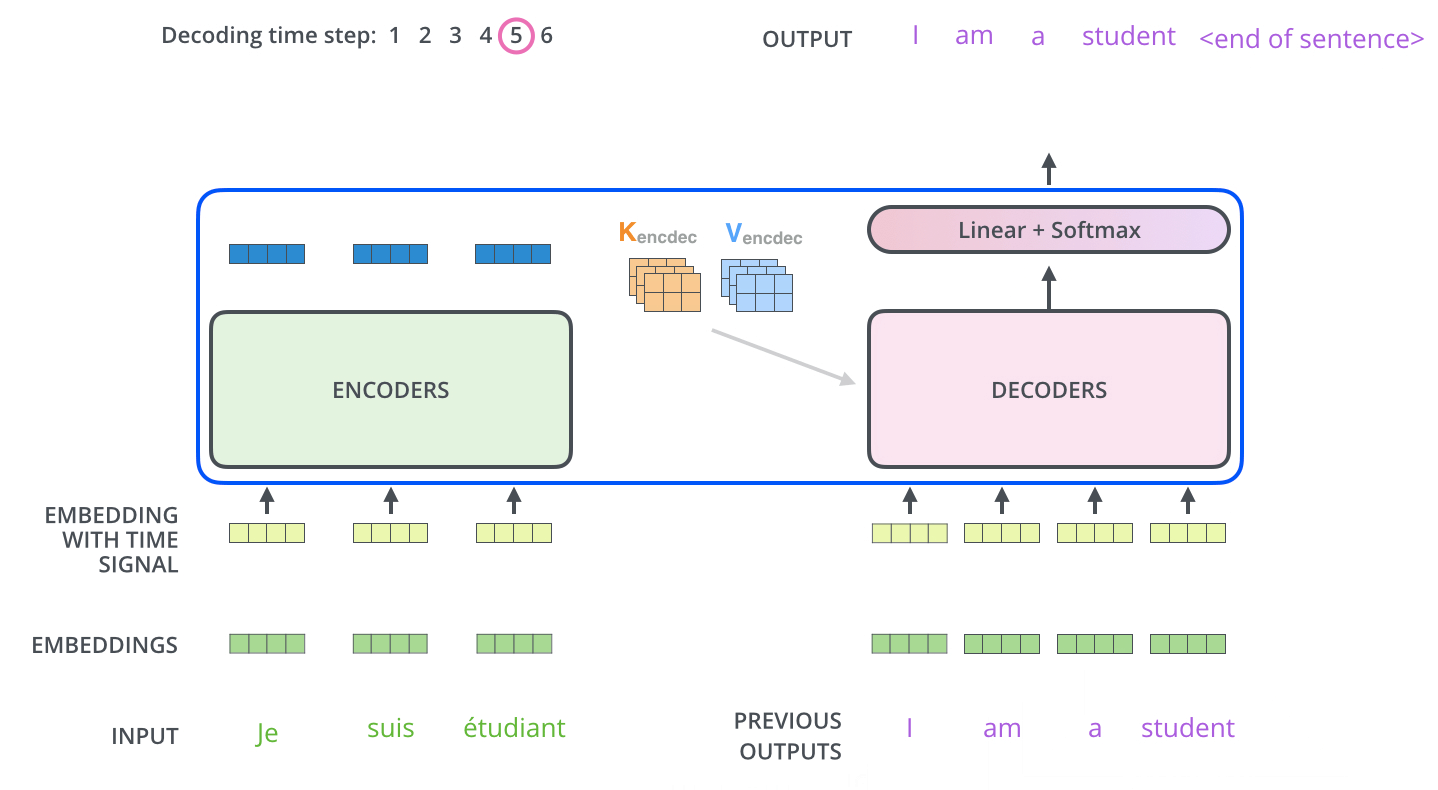
\includegraphics[width=0.5\textwidth]{image/transformer_decoding_2.png}
\end{figure}

解码器中的自注意力层的工作方式与编码器中的有所不同:

在解码器中,自注意力层只能关注输出序列中已经出现的位置。这是通过在自注意力计算的 softmax 步骤之前,将未来的位置屏蔽(设置为 `-inf`)来实现的。

“编码器 - 解码器注意力”层的工作原理类似于多头自注意力,不同之处在于它从下方的层中获取查询矩阵,并使用编码器堆栈输出的键和值矩阵。

\section{最终的线性层和 Softmax 层 (Softmax Layer)}

解码器堆栈的输出是一个浮点向量,我们怎样将这个向量转换为一个单词呢?这正是最后一个线性层的职责,该层后面紧接着一个 Softmax 层 (Softmax Layer)。

线性层其实就是一个简单的全连接神经网络,它的作用是将解码器堆栈输出的向量转换为一个更大的向量,称为 logits 向量 (logits vector)。

假设我们的模型掌握了从训练数据集中学习到的 10,000 个不同的英语单词(即模型的“输出词汇”)。这将使得 logits 向量的宽度达到 10,000 个单元,每个单元对应一个独特单词的得分。这就是我们如何理解经过线性层处理后模型的输出结果。

接下来,Softmax 层会将这些分数转化为概率值(所有概率值都是正数,且总和为 1.0)。概率值最高的单元被选出,与之对应的单词就是该时间步骤的输出结果。

\begin{figure}[ht]
	\centering
	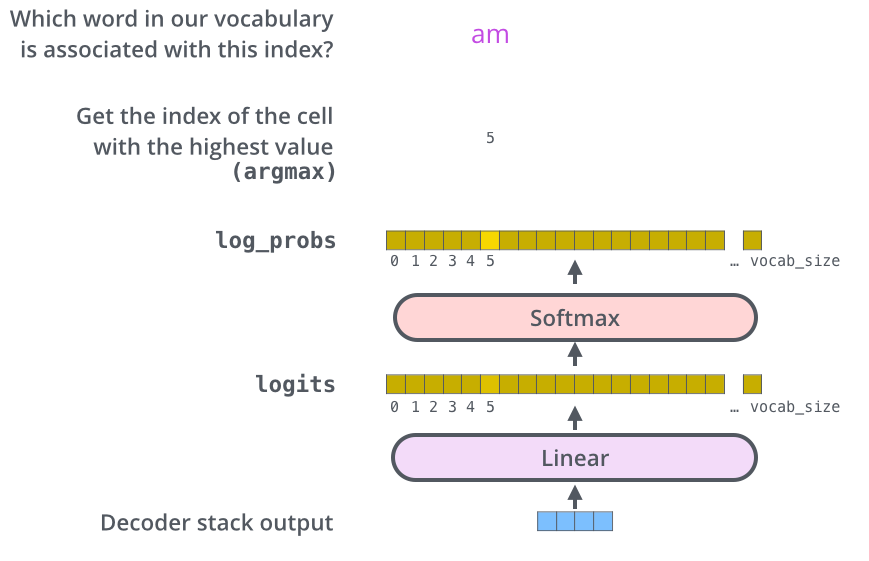
\includegraphics[width=0.5\textwidth]{image/transformer_decoder_output_softmax.png}
\end{figure}

此图展示了从解码器堆栈输出的向量开始,最终如何转换成一个输出单词的过程。

\section{训练回顾}

现在我们已经了解了通过一个训练过的 Transformer 模型进行的完整前向传播过程,不妨回顾一下训练模型的基本思路。

在训练期间,一个未经训练的模型将执行与上述相同的前向传播过程。但由于我们是在有标签的训练数据集上进行训练,因此我们能够将模型的输出与实际正确的输出进行对比。

为了更直观地理解,假设我们的输出词汇表仅包含六个单词:“a”, “am”, “i”, `“thanks”, “student”和“<eos>”(代表“句子结束”)。

\begin{figure}[ht]
	\centering
	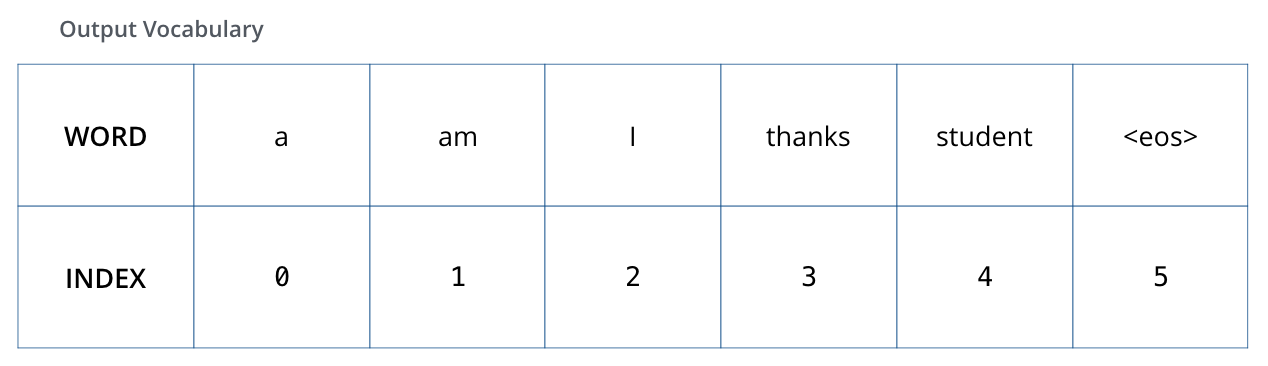
\includegraphics[width=0.5\textwidth]{image/vocabulary.png}
\end{figure}

我们模型的输出词汇表是在训练开始前的预处理阶段创建的。

定义输出词汇表后,我们可以用同宽度的向量来标识词汇表中的每个单词,这种方法称为 one-hot 编码。例如,我们可以用以下向量来表示单词“am”:
\begin{figure}[ht]
	\centering
	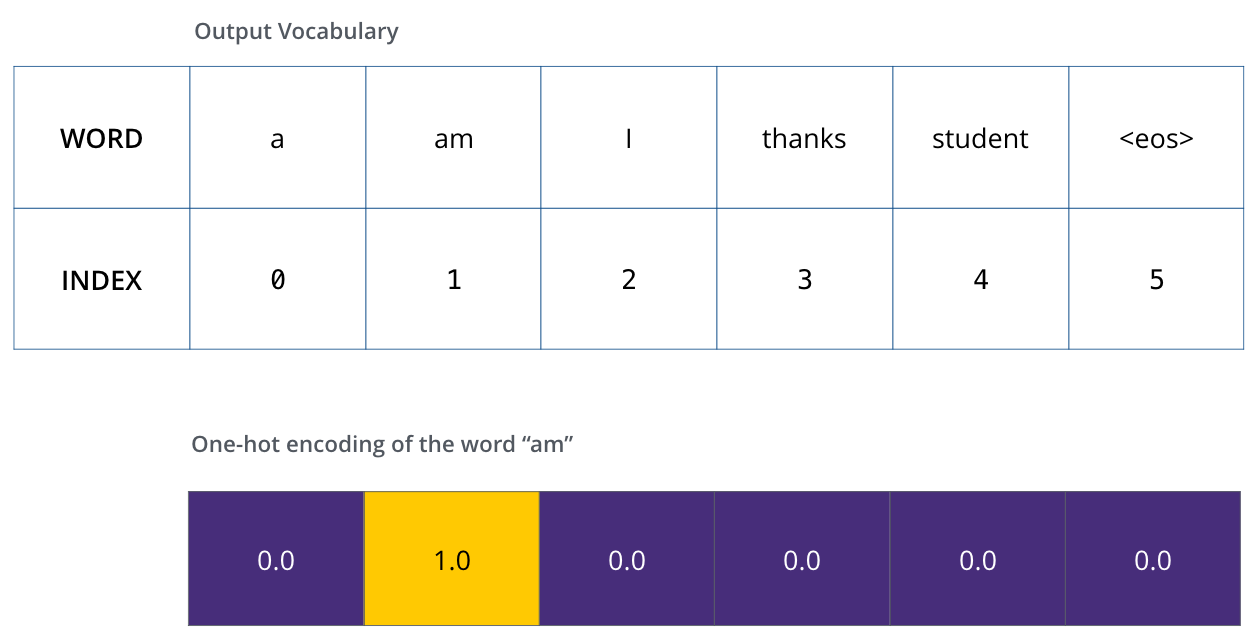
\includegraphics[width=0.5\textwidth]{image/one-hot-vocabulary-example.png}
\end{figure}

示例:展示了我们输出词汇表的 one-hot 编码方式

在回顾这些内容之后,我们来讨论模型的损失函数,这是我们在训练阶段优化的指标,目的是培养出一个训练有素且极为精确的模型。

\section{损失函数}

设想我们在训练一个模型,而这是训练初期的第一步。我们用一个基本的例子来进行训练:将“merci”译为“thanks”。

这意味着我们想得到一个输出,它以概率分布的形式表示“thanks”。但鉴于模型尚未训练完全,这种情况不会马上出现。
\begin{figure}[ht]
    \centering
    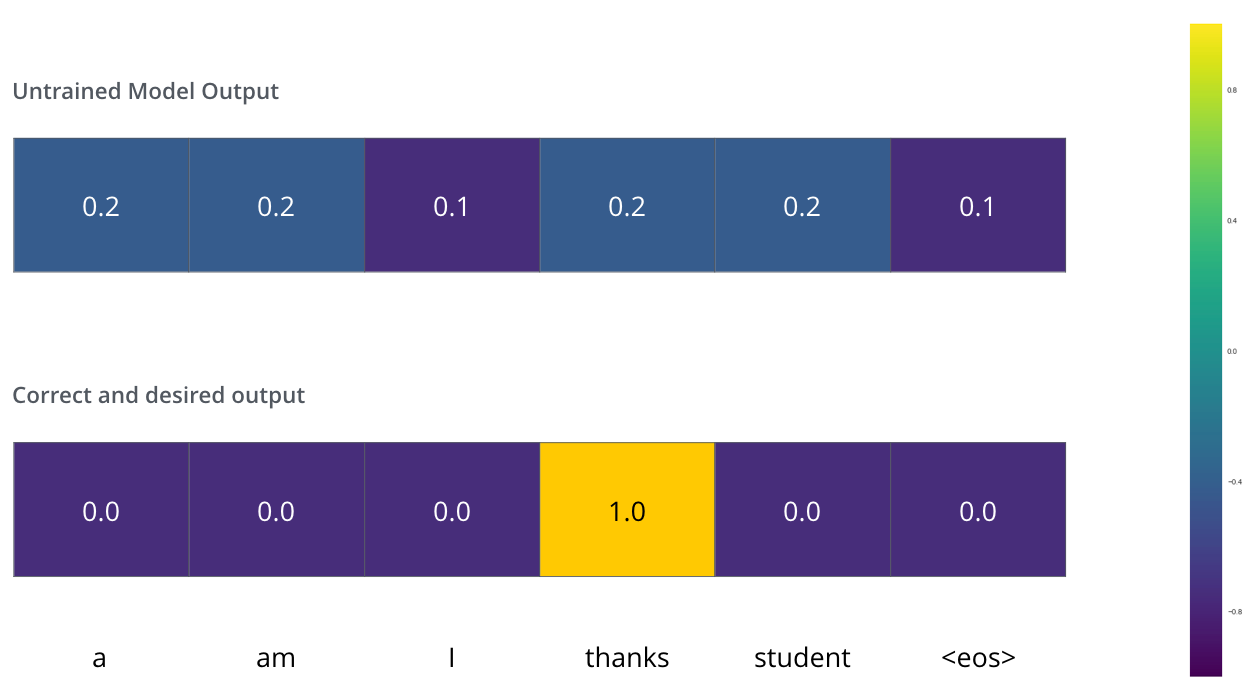
\includegraphics[width=0.5\textwidth]{image/transformer_logits_output_and_label.png}
\end{figure}

由于模型的参数(权重)是随机设定的,一个未经训练的模型会为每个词生成一个任意值的概率分布。我们可以将这个分布与实际的输出相比较,然后通过反向传播调整模型的所有权重,让输出更贴近我们的目标。

如何比较两个概率分布呢?我们可以简单地做差运算。想了解更多,请查阅 \href{https://colah.github.io/posts/2015-09-Visual-Information/}{交叉熵} 和 \href{https://www.countbayesie.com/blog/2017/5/9/kullback-leibler-divergence-explained}{Kullback-Leibler 散度}。

但这只是一个简化的例子。更实际的情况是,我们会用一个长于单词的句子来训练。比如,输入:“je suis étudiant”,期望输出:“i am a student”。我们实际上希望模型依次产生一系列概率分布,其中:

\begin{itemize}
    \item 每个分布都是一个宽度等于词汇表大小(vocab\_size)的向量(在我们的例子中是 6,但实际上可能是 30,000 或 50,000)
    \item 第一个概率分布中,“i”对应的单元格概率最高
    \item 第二个概率分布中,“am”对应的单元格概率最高
    \item 以此类推,直到第五个输出分布标志着``\texttt{<end of sentence>}``,这也是词汇表中的一个词。
\end{itemize}

\begin{figure}[ht]
    \centering
    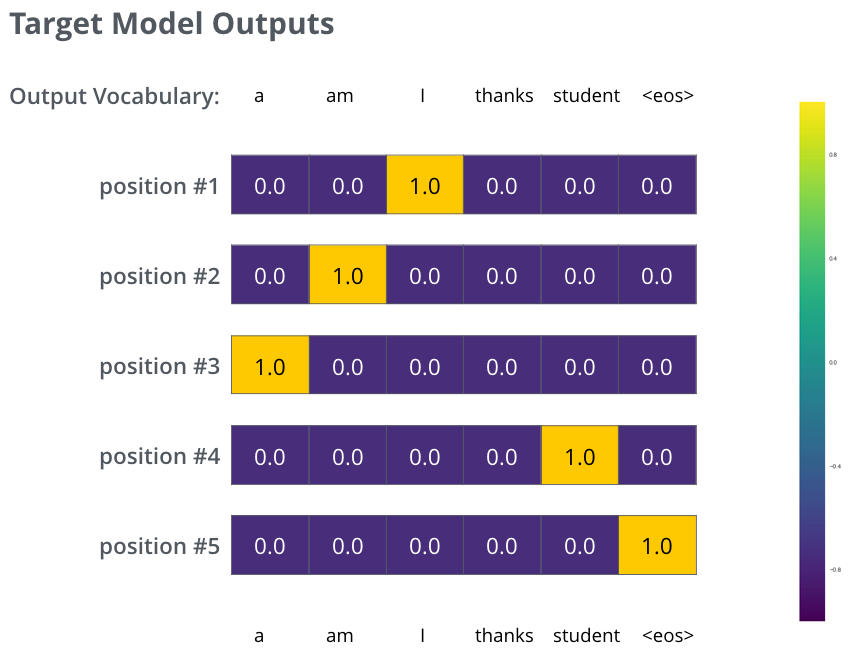
\includegraphics[width=0.5\textwidth]{image/output_target_probability_distributions.png}
\end{figure}

在一个样本句子的训练例子中,我们的目标是训练模型以获得这些特定的概率分布。

在对足够大的数据集进行了足够长时间的训练之后,我们希望模型生成的概率分布能够与这些目标分布相似。
\begin{figure}[ht]
	\vspace{-10mm}
    \centering
    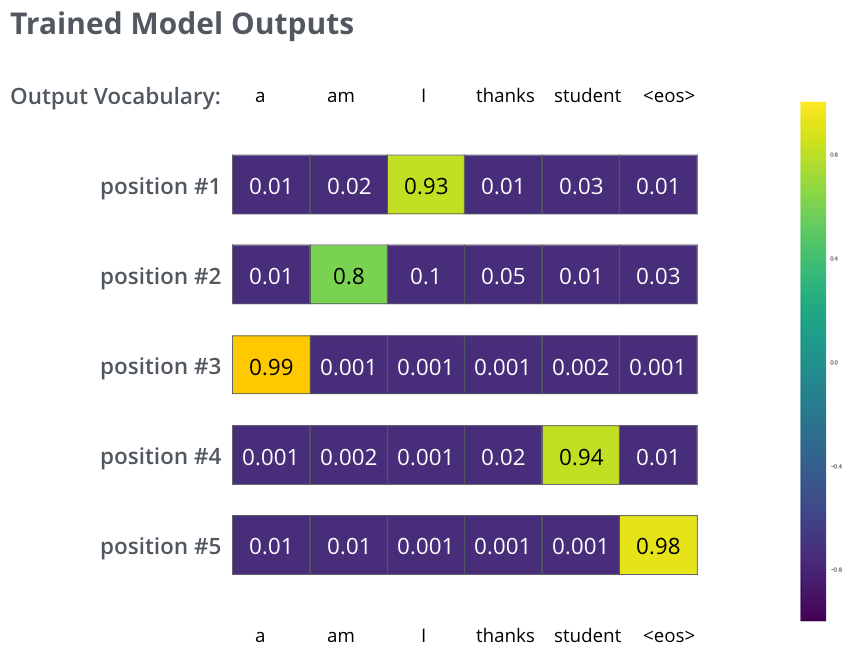
\includegraphics[width=0.5\textwidth]{image/output_trained_model_probability_distributions.png}
\end{figure}

我们期待,经过训练的模型能够给出我们所期望的正确翻译。但如果这个短语原本就在训练数据集中(参见:\href{https://www.youtube.com/watch?v=TIgfjmp-4BA}{交叉验证}),那么这并不能说明太多。值得注意的是,即使在某些时间步骤中某个位置的输出概率很低,每个位置还是会有一定概率值 —— 这正是 softmax 函数的一个重要特性,它在训练过程中起到关键作用。

由于模型逐个产生输出,我们可以认为它会从概率分布中选出概率最高的单词,而舍弃其他选项。这就是一种称为贪婪解码的方法。另一种方法则是保留概率最高的前两个单词(例如 I 和 a),在下一步中,模型分别假设第一个输出位置是 I 和 a,运行两次。我们将根据位置 \#1 和 \#2 总体上产生的错误更少的版本进行保留。对于位置 \#2 和 \#3 等,我们重复这个过程。这种方法被称为“束搜索”(beam search),在我们的例子中,beam\_size 设定为两(意味着随时保留两个部分翻译的假设在内存中),top\_beams 也是两(即我们将得到两个翻译结果)。这些都是可以进行调整和实验的超参数。

\section{探索并理解 Transformer}

我希望这能成为你开始了解 Transformer 核心概念的一个有益起点。如果你想更深入地探索,我建议以下几个步骤:
\begin{itemize}
    \item 阅读 \href{https://arxiv.org/abs/1706.03762}{Attention Is All You Need} 论文,Transformer 博客文章(\href{https://ai.googleblog.com/2017/08/transformer-novel-neural-network.html}{Transformer: A Novel Neural Network Architecture for Language Understanding}),以及 \href{https://ai.googleblog.com/2017/06/accelerating-deep-learning-research.html}{Tensor2Tensor 公告}。
    \item 观看 \href{https://www.youtube.com/watch?v=rBCqOTEfxvg}{Łukasz Kaiser 的演讲},他在其中详细介绍了模型及其细节。
    \item 实践 \href{https://colab.research.google.com/github/tensorflow/tensor2tensor/blob/master/tensor2tensor/notebooks/hello_t2t.ipynb}{Tensor2Tensor 仓库提供的 Jupyter 笔记本}。
    \item 探索 \href{https://github.com/tensorflow/tensor2tensor}{Tensor2Tensor 仓库}。
\end{itemize}

值得关注的后续工作包括:
\begin{itemize}
    \item \textit{Depthwise Separable Convolutions for Neural Machine Translation}:探讨用于神经机器翻译的深度可分离卷积。
    \item \textit{One Model To Learn Them All}:介绍一种多功能模型,适用于多种不同的任务。
    \item \textit{Discrete Autoencoders for Sequence Models}:关于序列模型中使用离散自编码器的研究。
    \item \textit{Generating Wikipedia by Summarizing Long Sequences}:总结长序列以生成维基百科内容的方法。
    \item \textit{Image Transformer}:介绍了一种用于图像处理的 Transformer 模型。
    \item \textit{Training Tips for the Transformer Model}:提供了训练 Transformer 模型的技巧。
    \item \textit{Self-Attention with Relative Position Representations}:讨论了自注意力机制中的相对位置表示。
    \item \textit{Fast Decoding in Sequence Models using Discrete Latent Variables}:使用离散潜变量加速序列模型的解码过程。
    \item \textit{Adafactor: Adaptive Learning Rates with Sublinear Memory Cost}:介绍了一种具有次线性内存成本的自适应学习率方法。
\end{itemize}









%\printbibliography[heading=bibintoc, title=\ebibname]

\end{document}
